\chapter{Consistency through different transcriptomics studies with RNA-Seq}
\label{ch:Transcriptomics}

\section{introduction}
Why?

\begin{itemize}
    \item Difficulty of sampling of normal conditions for human, particularly
        for the solid tissues. (could be very useful in case of cancer for
        example)
    \item Lots of transcriptomics data in the repository of EBI. Can we use
        this as a base for reference?
    \item previous point not new, but recently multiplications of studies on
        normal human studies based on \Rnaseq
    \item Indeed, in the past people tried with microarray data but didn't work
        \TK{find sources}
    \item When I started this study, there wasn't any publication on this matter
        yet, but \Rnaseq was considered as quantitative (when microarrays were
        considered semi-quantitative at best).
    \item nobody did published on my specific subject yet, but since then things changed
    \item first paper from MACQ/SEC III
    \item increasing number of papers that been published on the subject
    \item I will discuss the different part of the papers that are relevant
        with additions on what my study confirms/refutes or expands them.
\end{itemize}

While current high-throughput gene expression studies are mainly about
differential gene expression between conditions, healthy controls are not always
enough or even available.
Although, many atlases have been released to help on this issue,
there is still not any direct method that would allow you more than check the
presence (or lack of detection) of specific genes in a given condition.

With the increasing number of studies of normal tissues with overlapping conditions
\cref{fig:VennStudiesT}, we are investigating the consistency of gene-tissue
associations on
one side but moreover we would like to assess the expression levels across the
datasets in the aim of integrating all the available data in a gene expression
baseline reference.

When I started this project there was not any study, comprehensive or not, that
was investigating in-depth the consistency of transcriptome expression measurements
for one condition across studies.


As previously stated in the introduction, while I started this project,
there wasn't any study that was investigating in-depth the reproducibility of
transcriptomics.

However, in August 2014 a paper comparing different preparation methods,
sequencing technologies operated in different laboratories
on samples from the same biological source concludes that while absolute
measurements are not consistent, the relative expression is highly consistent
(95\% Pearson correlation?)


\section{Available studies}
\label{sec:Trans_AvailableStudies}

All the datasets with which I worked are fitting three main criteria.
They comprise human normal samples from at least three kind of tissues.
They have been sequenced with \Rnaseq\ and
the \emph{raw} data is available and reuseable.
While they are quite a few more studies that I would have like to use
this last point was often the critical reason why they have not been included.
Indeed, many times I encountered data with ambiguous encoding format and as the
studies were a little bit outdated,
I also could not get the answer from the original authors.

I describe hereafter the datasets in the chronological order of their first
publication.
When I started this work in 2013, there were only three complying
datasets at that time. Fortunately, I was later
able to incorporate two other datasets to my study. One of them is the \Gtex\
pilot (version 1.4) data and the other one is the Uhlén et al.\ dataset (first
published in 2014 and then extended for the \citet{uhlen2014} paper).
The number of provided samples and covered tissues for these two datasets
is far greater than the other ones. These \dataset{\Gtex} and \dataset{Uhlén}
datasets are indeed presenting a greater set of common tissues. Moreover,
the more recent and similar technology used (either for the libraries preparation,
the sequencer or the paired-end protocols) and the studies design that includes
biological replicates for every tissue had motivated a more focused comparison
based only on these two datasets.


\subsection{Castle et al. dataset}

This dataset has been published along with the \paper{\citetitle{castleData}}
by \citet{castleData} who were interested to explore
with sequencing-based technology the whole RNA repertoire. They essentially
focused their study on the non coding part and found that
while \glspl{mRNA} could be highly tissue-specific, \glspl{ncRNA} have generally
greater tissue-specific expression patterns.

They used multiple-donors pooled tissues samples (purchased as total \gls{RNA})
and prepared the libraries following a whole transcriptomic protocol
\citep{Armour:2009}: where nonribosomal \gls{RNA} transcripts are
specifically amplified by \gls{PCR}.

They generated an average of 50 millions sequence reads per tissue
using an Illumina Genome Analyser-II sequencer (single-end).
They trimmed their original reads to 28 \gls{nt}
and released them through EMBL archives (\ENA{ERP000257}
and \ArrayExpress{E-MTAB-305}).

Despite several limitations (lack of replicates, old technology, small reads),
I used this dataset for two main reasons. It is the oldest available \Rnaseq\
data I found that was performed on Human normal tissues and it is comprising
\glspl{ncRNA}.


\subsection{Brawand et al. dataset}

In the corresponding article entitled \paper{\citetitle{VTpaper}},
\citet{VTpaper}~collected 6 organs from 10 different vertebrates:
9 mammalians (including Human) and a bird. They are focused on the
evolution of the mammalian transcriptomes -- while there were existing studies
on the matter, the sequencing approach was then creating new perspectives.

They have biological replicates: one male
and one female for the somatic tissue and two males for the testes samples.
They used a
polyA-selected protocol to prepare the libraries. Hence, the samples are largely
enriched in protein coding genes.

They generated an average of 3,2 billion reads of 76 base pairs per sample
using an Illumina Genome Analyser IIx (single-end) and they released them
through \gls{GEO} (accession number: GSE30352).
I personally retrieved the data from
\ArrayExpress{E-GEOD-30352}\footnote{ArrayExpress routinely imports
datasets from \gls{GEO} on a weekly basis.}.


\subsection{Illumina Body Map 2.0}

This dataset has been first created in 2010 and released in
2011\footnote{See: \citetitle{ibmEnsembl} - \cite{ibmEnsembl}} by Illumina
mostly to advertise its most recent technology improvement at that time:
the paired-end sequencing.
Until then, all the sequencing was done from only one end of the \gls{DNA} (or
\gls{RNA}) fragments\footnote{With a simple change in the library preparation protocol,
Illumina introduced the paired-end sequencing which present many improvements
over the previous protocol (single-end). One particular enhancement, the
detection of rearrangements, allows the detection of gene fusions and
novel splicing isoforms. For this reason, most of the following transcriptome
studies based on \Rnaseq\ are using paired-end sequencing.}.

The first published paper to analyse this dataset was done by
\citet{ibmrelatedpaper}: \paper{\citetitle{ibmrelatedpaper}}.
It was referenced many times since then as it was for a couple of years
the most extensive freely available \Rnaseq\ dataset of human tissues.

It comprises 16 tissues (one donor per tissue), which were prepared with a
polyA-selected library preparation protocol and then have been sequenced once
with a singled-end protocol and then a second time with a paired-end one. There
are some added libraries which have been created by mixing together the 16 tissues.

The sequencing was performed with a HiSeq 2000.

I retrieved this dataset from \ArrayExpress{E-MTAB-503} (\ENA{ERP000546}).

\begin{comment}
\rough{Dataset: \begin{itemize}
        \item why?
        \item Main findings (particularly the ones that impact me)
        \item how they created it
\end{itemize}}
\end{comment}

\subsection{Uhlén et al. dataset}


\subsection{Gtex data}


\begin{figure}%[!htbp]
    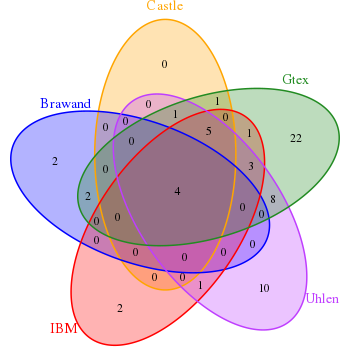
\includegraphics[scale=0.8]{transcriptomics/VennStudiesT}\centering
    \caption[Distribution of unique and shared tissues between the
    transcriptomic datasets]%
    {\label{fig:VennStudiesT}\textbf{Distribution of unique and shared tissues
    between the transcriptomic datasets}}
\end{figure}


\subsection{Overview of the analysis}

The main characteristics of the different datasets are summarised
in~\cref{tab:Trans5DF}.


\begin{sidewaystable}
    \centering
    \caption{\label{tab:Trans5DF}Technical description of the 5 transcriptomic
    dataset (\Rnaseq)
     used for this study}
\begin{tabular}{@{}cccccccccc@{}}
\toprule
\multicolumn{1}{c|}
    {\multirow{2}{*}{ArrayExpress ID}} &
     \multicolumn{1}{c|}{\multirow{2}{*}{Data ID}} &
     \multicolumn{2}{c|}{\begin{tabular}[c]{@{}c@{}}Library\\Preparation\end{tabular}} &
     \multicolumn{2}{c|}{Sequencing} &
     \multicolumn{2}{c|}{Replicates} &
     \multicolumn{1}{c|}{\multirow{2}{*}{\begin{tabular}[c]{@{}c@{}}Tissue\\
             Number\end{tabular}}} &
     \multirow{2}{*}{\begin{tabular}[c]{@{}c@{}}Multi-sampling\\ from the \\ same individual\end{tabular}} \\
     \cmidrule(lr){3-8}
     \multicolumn{1}{c|}{} & \multicolumn{1}{c|}{} &
     \multicolumn{1}{c|}{\begin{tabular}[c]{@{}c@{}}Whole\\ RNA\end{tabular}} &
     \multicolumn{1}{c|}{\begin{tabular}[c]{@{}c@{}}PolyA\\ selected\end{tabular}} &
     \multicolumn{1}{c|}{\begin{tabular}[c]{@{}c@{}}Single\\ end\end{tabular}} &
     \multicolumn{1}{c|}{\begin{tabular}[c]{@{}c@{}}Paired\\ end\end{tabular}} &
     \multicolumn{1}{c|}{Biological} & \multicolumn{1}{c|}{Technical} &
     \multicolumn{1}{c|}{} &  \\
\midrule
E-MTAB-305 & Castle & Y &  & Y &  &  &  & 11 &  \\
E-GEOD-30352 & Brawand &  & Y & Y &  & Y &  & 8 &  \\
E-MTAB-513 & IBM &  & Y & Y & Y &  & (Y) & 16 &  \\
E-MTAB-2836 & Uhlén &  & Y &  & Y & Y & Y & 32 &  \\
E-MTAB-2919 & Gtex  &  & Y &  & Y & Y &  & 54 & Y \\
\bottomrule
\end{tabular}
\end{sidewaystable}

\section{Consistency of processing methodology}\label{sec:Trans_consistentMethodo}

    \subsection{Reuse of processed data issues}\label{subsec:Trans_reuseOfData}

    \subsection{Genome build and annotation impact}\label{subsec:Trans_AnnotImpact}

\section{Results}\label{sec:Trans_Results}

RNA-seq is consistent across datasets; samples are more likely to cluster by
biological origins than by studies. (Figure 2)
While Pearson correlations are higher, without any a priori Spearman correlations
allow a better separation of the different tissues in distinct clusters across
datasets.

Many genes have a consistent profile of expression levels through the different
datasets.
To help EBI Expression Atlas has developed a feature that allows the visualisation
of the expression of a gene (or protein) across the different dataset that it
integrates. (Figure 3)

Reuse of data allows the assessment of the biological quality of a sample.
While RNA-seq workflows integrate numerous quality checks for their different steps,
it is not always easy to appraise the original quality of the samples. Comparing
similar conditions from different sources allow some high level biological check.
Indeed, we noticed that some tissues have a more unique profile in specific
datasets.

Overall gene expressions for protein coding genes across different tissues
correlated highly between datasets. (See part 3. Integration of Transcriptomics
and Proteomics studies – Figure 15)



    \subsection{Reproducibility of expression profile at tissue level}\label{subsec:Trans_ReproExpresTissue}

        \subsubsection{Correlation}\label{subsubsec:Trans_Tissue_Corr}
        \subsubsection{Clustering}\label{subsubsec:Trans_Tissue_cluster}

    \subsection{Reproducibility of expression profile at gene level}\label{subsec:Trans_ReproExpresGene}

    \subsection{Tissue specific,housekeeping genes and other categories}\label{subsec:Trans_TissueSpeAndHK}

    \subsection{Curated sets}\label{subsec:Trans_curatedSets}

\section{Discussion}\label{sec:Trans_discussion}



\begin{comment}
  \begin{figure}%[!htbp]
      \includegraphics%[scale=0.6]%
      {transcriptomics/}\centering
      \caption[]
      {\label{fig:}\textbf{}}
  \end{figure}
\end{comment}
